\chapter{Laboratorio 5}
Il primo circuito realizzato in questa esperienza di laboratorio permette di effettuare lo switch debouncing attraverso l'integrato LM555. Nella figura \ref{fig:circuito_1} è riportato lo schema del circuito.
\begin{figure}[h!]
	\centering
	\begin{minipage}{.45\textwidth}
		\scalebox{.47}{
			\begin{circuitikz}
				%Main dip package
				\draw (0,0) node[dipchip,num pins=8, hide numbers, external pins width=0.1, scale=3, external pad fraction=6](C){LM555};
				%Pin names
				\node [right] at (C.bpin 1) {GND};
				\node [right] at (C.bpin 2) {Trigger};
				\node [right] at (C.bpin 3) {Output};
				\node [right] at (C.bpin 4) {Reset};
				\node [left] at (C.bpin 5) {Control Voltage};
				\node [left] at (C.bpin 6) {Threshold};
				\node [left] at (C.bpin 7) {Discharge};
				\node [left] at (C.bpin 8) {$V_{CC}$};
				%Connections
				\draw (C.pin 1) -- ++(-2.9,0) ++(-.1,0) node[jump crossing](crgnd){} ++(-.1,0) -- ++(-.9,0) -- ++(0,-6) node[ground]{};
				\draw (C.pin 8) -- ++(2,0) coordinate(vcc) -- ++(0,1.35) node[vcc]{$V_{CC}$};
				\draw (C.pin 7) -- ++(2,0) coordinate(dsc) to[R=$R$] (vcc);
				\draw (C.pin 6) -- ++(2,0) coordinate(trs) -- (dsc);
				\draw (trs) -- ++(2,0) to[C=$C$] ++(0,-2.68) node[ground]{};
				\draw (C.pin 5) -- ++(2,0) to[C=$C_2$] ++(0,-1) node[ground]{};
				\draw (C.pin 4) -- ++(-1.5,0) -- ++(0,3) to[crossing] ++(0,.72) to[crossing] ++ (0,2.64) node[vcc]{$V_{CC}$};
				\draw (C.pin 3) to[short, -o] ++(-1,0) ++(0,.1) node[above]{$v_{out}$};
				\draw (C.pin 2) -- ++(-3,0) coordinate(vin);
				\draw (vin) to[nopb=$B$] ++(0,-4.32) node[ground]{};
				\draw (vin) to[R=$R_2$] (crgnd) -- ++(0,1.33) node[vcc]{$V_{CC}$};
				\draw[thick] (-7.5,-5.3) rectangle (8,5.9);
			\end{circuitikz}
		}
	\end{minipage}\qquad
	\begin{minipage}{.45\textwidth}
		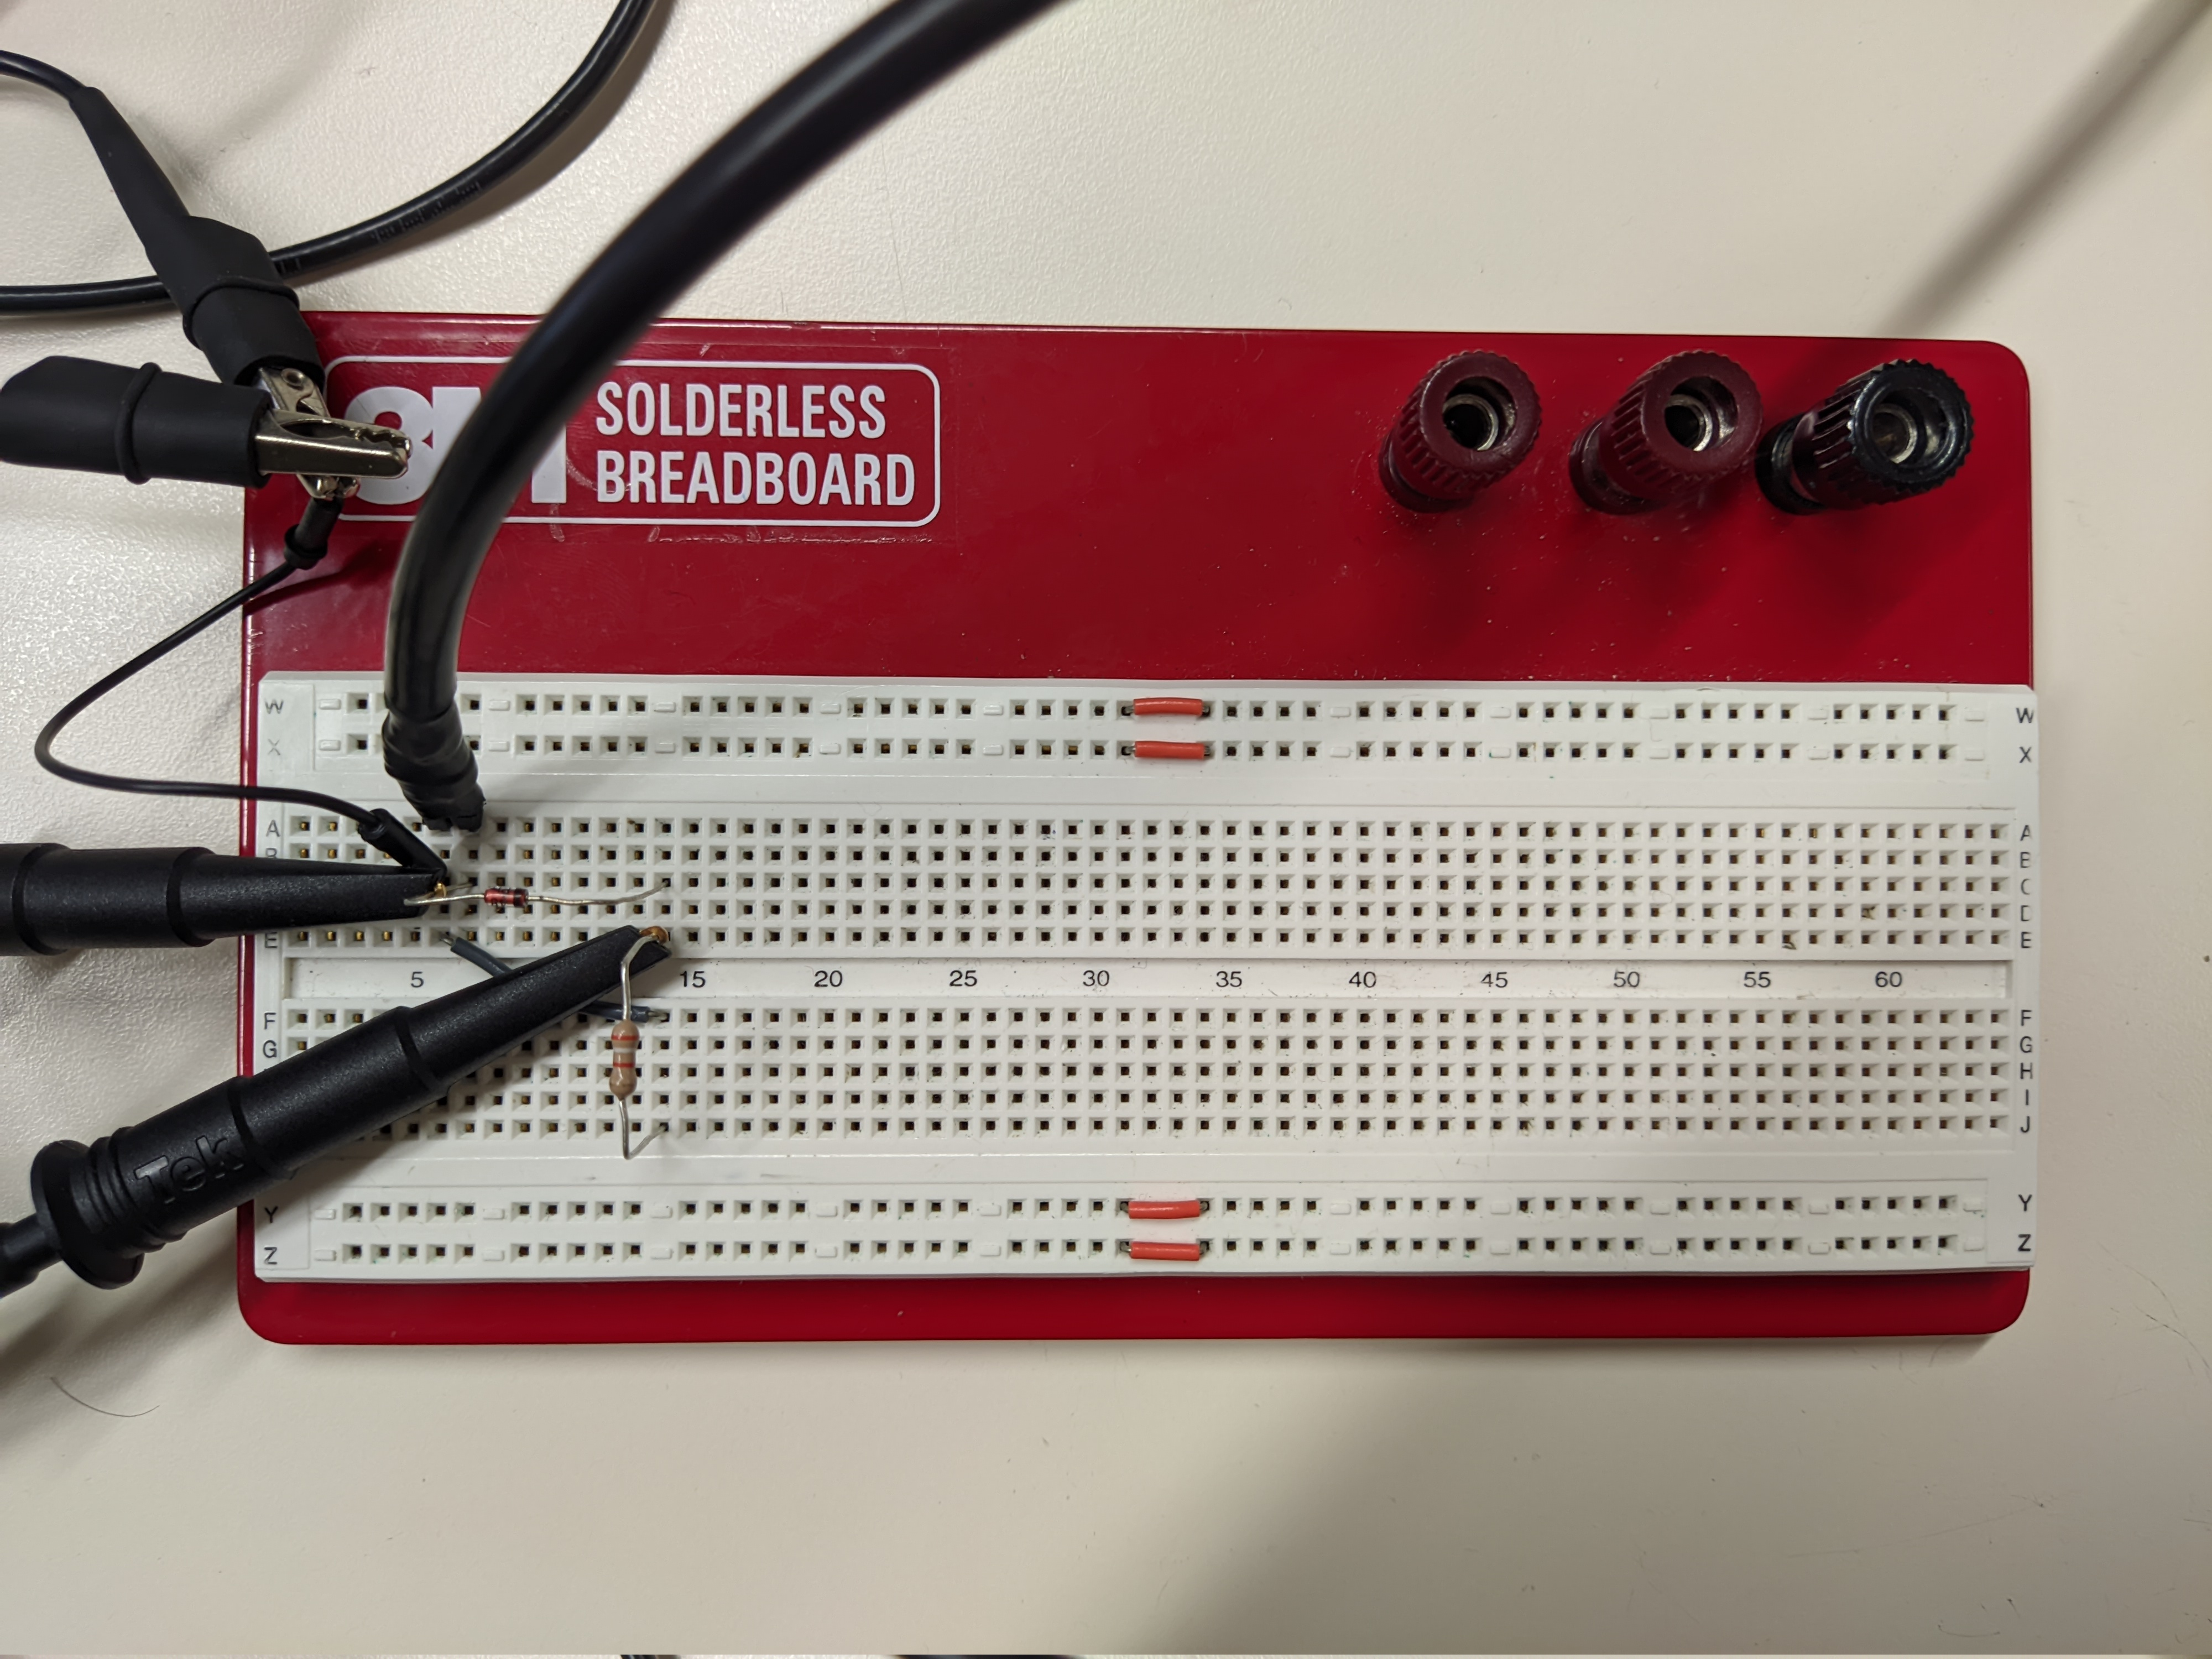
\includegraphics[width=\linewidth]{./ImageFiles/Laboratorio 5/CIR1.jpg}
	\end{minipage}
	\caption{Schema circuitale e foto del circuito realizzato.}
	\label{fig:circuito_1}
\end{figure}

\noindent
In questo circuito il Timer 555 è utilizzato in configurazione monostabile. A differenza del circuito realizzato nella relazione precedente, il segnale di trigger viene generato non più tramite il generatore di forme d'onda ma tramite un pulsante meccanico normalmente aperto. 
Esso ha un terminale connesso alla resistenza $R_2$ di pull-up verso $V_{CC}$, mentre l'altro terminale è connesso a massa. Per cui, quando l'interruttore è aperto sul nodo di \textit{Trigger} viene mantenuta una tensione di $V_{CC}$ grazie alla resistenza $R_2$. Quando l'interruttore viene chiuso invece il morsetto di \textit{Trigger} viene collegato a massa.  






Il problema dello switch bouncing\todo{altra bruttura} deriva dalla sua struttura meccanica interna. Infatti, quando questo viene chiuso o aperto, proprio per come è costruito internamente, questo tende ad oscillare per un certo periodo causando un "treno" di impulsi che vengono visti dall'elettronica davanti come un set continuo di pressioni e rilasci invece che una pressione singola come invece avviene nella realtà. Questo tipo di circuito quindi si comporta come da "filtro" per questo comportamento, fornendo in uscita solo il primo cambio di pendenza sul piedino del trigger invece di tutti gli eventi spuri generati all'ingresso, visto che la durata dell'evento di uscita è determinato puramente da R e da C e non dal numero di impulsi all'ingresso del 555.